% !TEX encoding = UTF-8
% !TEX TS-program = pdflatex
% !TEX root = ../tesi.tex

%**************************************************************
\chapter{Conclusioni}
\label{cap:conclusioni}
%**************************************************************

%**************************************************************
\section{Consuntivo}
Questa sezione descrive i risultati dello stage sotto forma di metriche. Nel complesso, il progetto è stato concluso con successo.
\subsection{Requisiti soddisfatti}
L'applicazione soddisfa tutti i requisiti\ref{tab:requisiti-funzionali} obbligatori (17/17) e la maggior parte dei requisiti desiderabili (5/6). Il requisito desiderabile non implementato, per questioni di tempo, è RD-6, ovvero esporre l'applicazione attraverso un'API. Implementerò questo requisito in un breve periodo di post-stage in azienda.
\label{tab:requisiti-resoconto}
\begin{longtable}{|l l|}
\caption{requisiti soddisfatti}\\
\hline
\textbf{Requisito} & \textbf{Risultato} \\
\hline
\endhead
RO-1     & soddisfatto\\
RO-2     & soddisfatto\\
RO-3     & soddisfatto\\
RO-3.1   & soddisfatto\\
RO-3.2   & soddisfatto\\
RO-3.3   & soddisfatto\\
RO-3.4   & soddisfatto\\
RO-4     & soddisfatto\\
RO-4.1   & soddisfatto\\
RO-4.2   & soddisfatto\\
RO-4.3   & soddisfatto\\
RO-4.4   & soddisfatto\\
RO-4.5   & soddisfatto\\
RO-4.6   & soddisfatto\\
RO-5     & soddisfatto\\
RO-6     & soddisfatto\\
RO-7     & soddisfatto\\
RD-1     & soddisfatto\\
RD-2     & soddisfatto\\
RD-3     & soddisfatto\\
RD-4     & soddisfatto\\
RD-5     & soddisfatto\\
RD-6     & non soddisfatto\\
\hline
\end{longtable}

\subsection{Metriche del codice}
\subsubsection*{Code coverage}
Il \textit{code coverage} è parti all'87\%. I metodi non coperti sono molto semplici e non necessitano di essere testati. 
\begin{figure}[H]
    \centering
    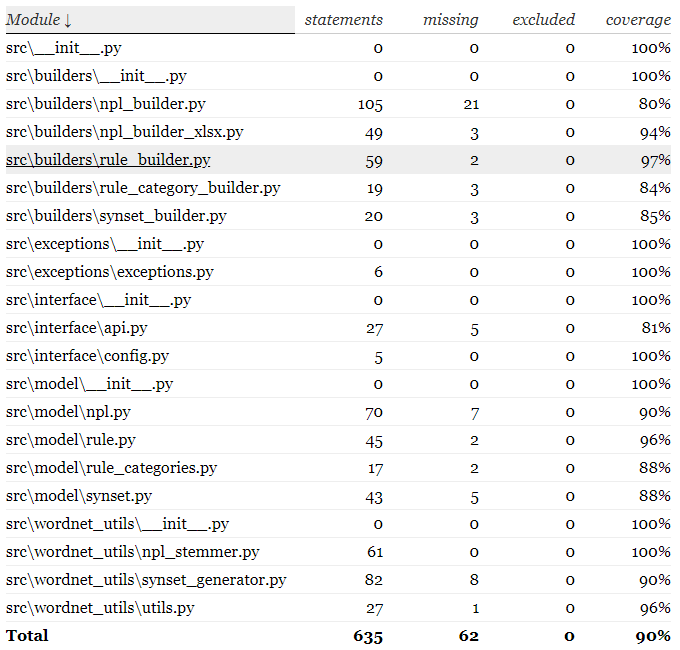
\includegraphics[width=0.8\columnwidth]{results/coverage.PNG} 
    \caption{code coverage}
    \label{coverage}
\end{figure}
\subsubsection*{Analisi statica}
Durante la codifica, ho utilizzato \textit{pycodestyle} per rispettare lo stile definito da PEP8. Questo ha portato a un codice privo di \textit{warning} rilevati da questa applicazione.
\begin{figure}[H]
    \centering
    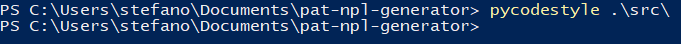
\includegraphics[width=0.9\columnwidth]{results/nostyle.PNG} 
    \caption{pycodestyle}
    \label{coverage}
\end{figure}
%**************************************************************
\section{Raggiungimento degli obiettivi}

%**************************************************************
\section{Conoscenze acquisite}
\begin{itemize}%TODO%
    \item \textbf{python};
    \item ho potuto imparare nella pratica come funziona una \textit{software house}, iniziando ad acquisire la professionalità richiesta per questo ambiente;
    \item ho imparato l'importanza e il ruolo del \textit{pre-processing} dei dati, prima di essere elaborati da un algoritmo di machine learning. Nel mondo reale, i dati sono pochi e preziosi, quindi è necessario sfruttarli al massimo e assicurarsi che l'output dell'algoritmo di \textit{machine learning} sia filtrato e analizzato, prima di essere esposto agli utenti del servizio.\\ Questo si contrappone con l'esperienza universitaria, dove il focus principale viene posto sul metodo, invece che sul risultato.
\end{itemize}
%**************************************************************
\section{Valutazione personale}
